\chapter{Proposed Sintactic and Semantic Analyzer}
\label{ch:proposed-sintactic-semantic-analyzer}

Once all the objectives and requirements to be achieved have been described,
the different systems and techniques existing to achieve them have been studied,
and their contributions and shortcomings have been evaluated, we will describe
the proposed solution both in terms of design and possible implementation

\section{Structure}
The system is divided into components so that each component works on its input
and produces its output. In this way, a parser is achieved that behaves like
an API where each element can be called individually. \cref{fig:shex-lite-sema}
shows the different components of this analyzer.

\begin{figure}
    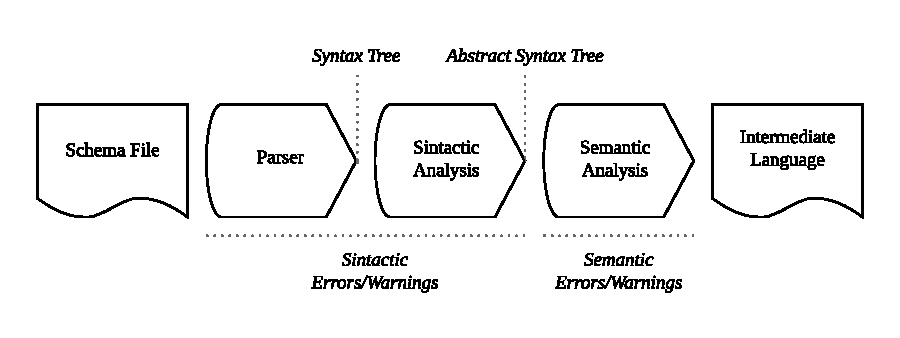
\includegraphics[width=\textwidth]{images/sin-sem-structure.pdf}
    \centering
    \caption[Sintactic and Semantic Analyzer structure]{Sintactic and Semantic Analyzer structure.}
    \label{fig:shex-lite-sema}
\end{figure}

\subsection{Parser}
We define the parsing stage as the process that begins when we receive the source code that makes up
the schema until the moment we produce a syntax tree. Therefore it includes the conversion to tokens
by the lexer, the grouping of tokens in rules and later in a syntax tree by the parser.

The general idea of this stage is that you take the source code as input and build a syntactic tree with all
the possible information from the source code. This implies that the syntactic tree is not only made up of
abstract grammar, but also of separators, braces and keywords. \cref{fig:shex-lite-st} shows an example
of the first 20 nodes generated by the parser. There we can see this composition of separators, keywords, braces
and content.

\begin{figure}
    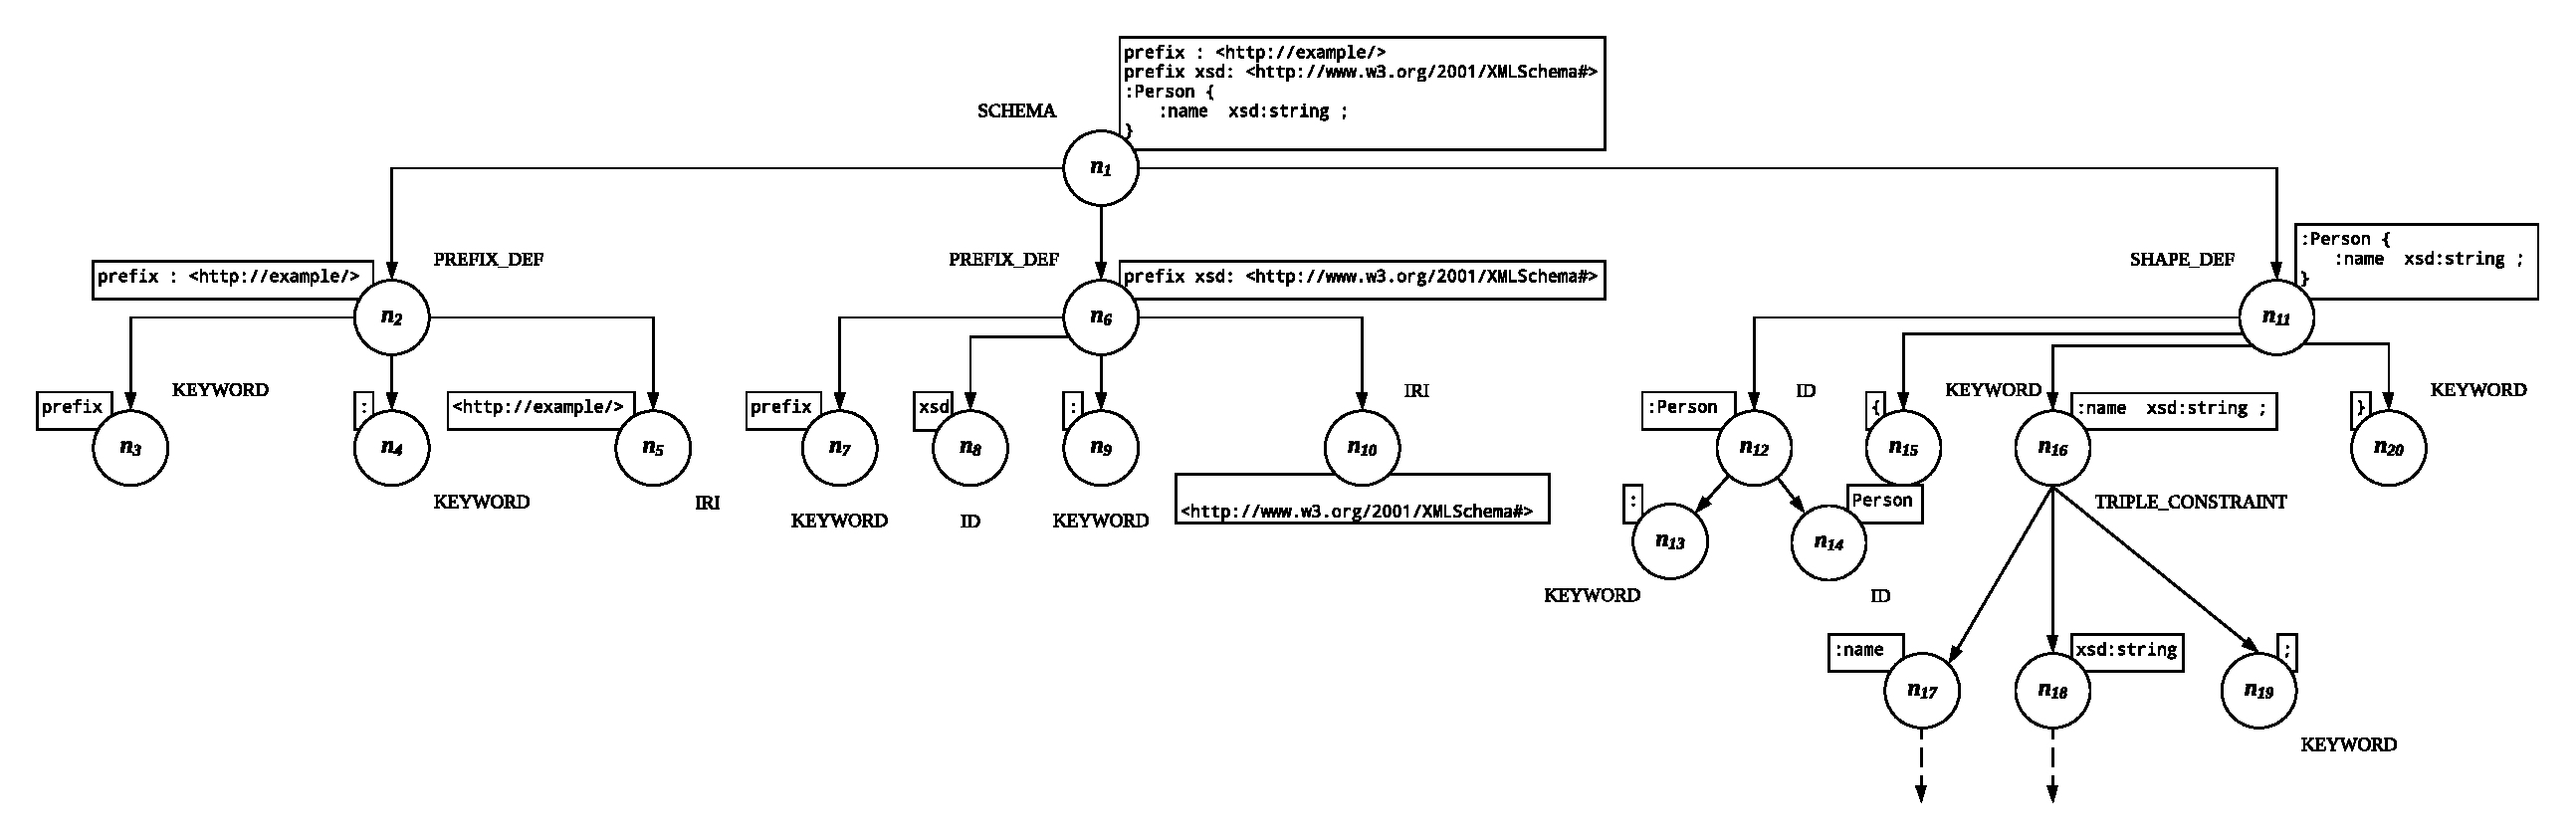
\includegraphics[width=\textwidth]{images/shex-lite-syntax-tree.pdf}
    \centering
    \caption[Syntax Tree tweenty first nodes produced by the parser]{Syntax Tree tweenty first nodes produced by the parser.}
    \label{fig:shex-lite-st}
\end{figure}

Once we have the complete syntactic tree generated, we can go through it to carry out syntactic analysis on the different elements.
For example, in the tree in \cref{fig:shex-lite-st} we could implement a validator that in the event that the last triple constraint
of a shape definition \textit{(node 16)} did not have the semicolon termination keyword \textit{(node 19)}, it would generate a
warning message to the user.

\subsection{Sintactic Analyzer}
The sintactic analyzer is in charge of traversing the syntactic tree in order to search for possible patterns that the user has to
be informed about. If none were found it would be understood that the syntactic tree is well formed and it will tranform the Syntax Tree
\cref{fig:shex-lite-st} into an Abstract Syntax Tree \cref{fig:shex-lite-sema-anal} \textit{(without the green and red relations)}.

For this, each node within our syntactic tree is aware of the context in which it is. Therefore we can ask questions to the nodes,
such as to a prefix definition \textit{(\cref{fig:shex-lite-st} $n_2$)}, do you have a label? \textit{(No)} or who is the node
that defines your iri? \textit{(node $n_5$)}. With questions like these, the syntactic tree can be analyzed for patterns that
represent warnings or errors.

\subsection{Semantic Analyzer}
The semantic analyzer is responsible of building all the possible relations between the AST nodes, analyze and check that
all those relations that must exist indeed exist. For this porpouse as just seen we reduce our Syntax Tree to an
Abstract Syntax Tree. \cref{fig:shex-lite-sema-anal} Shows a the resulting AST after the correspinding analysis and
transformations, we call this graph the \textit{Intermediate Language}.

\begin{figure}
    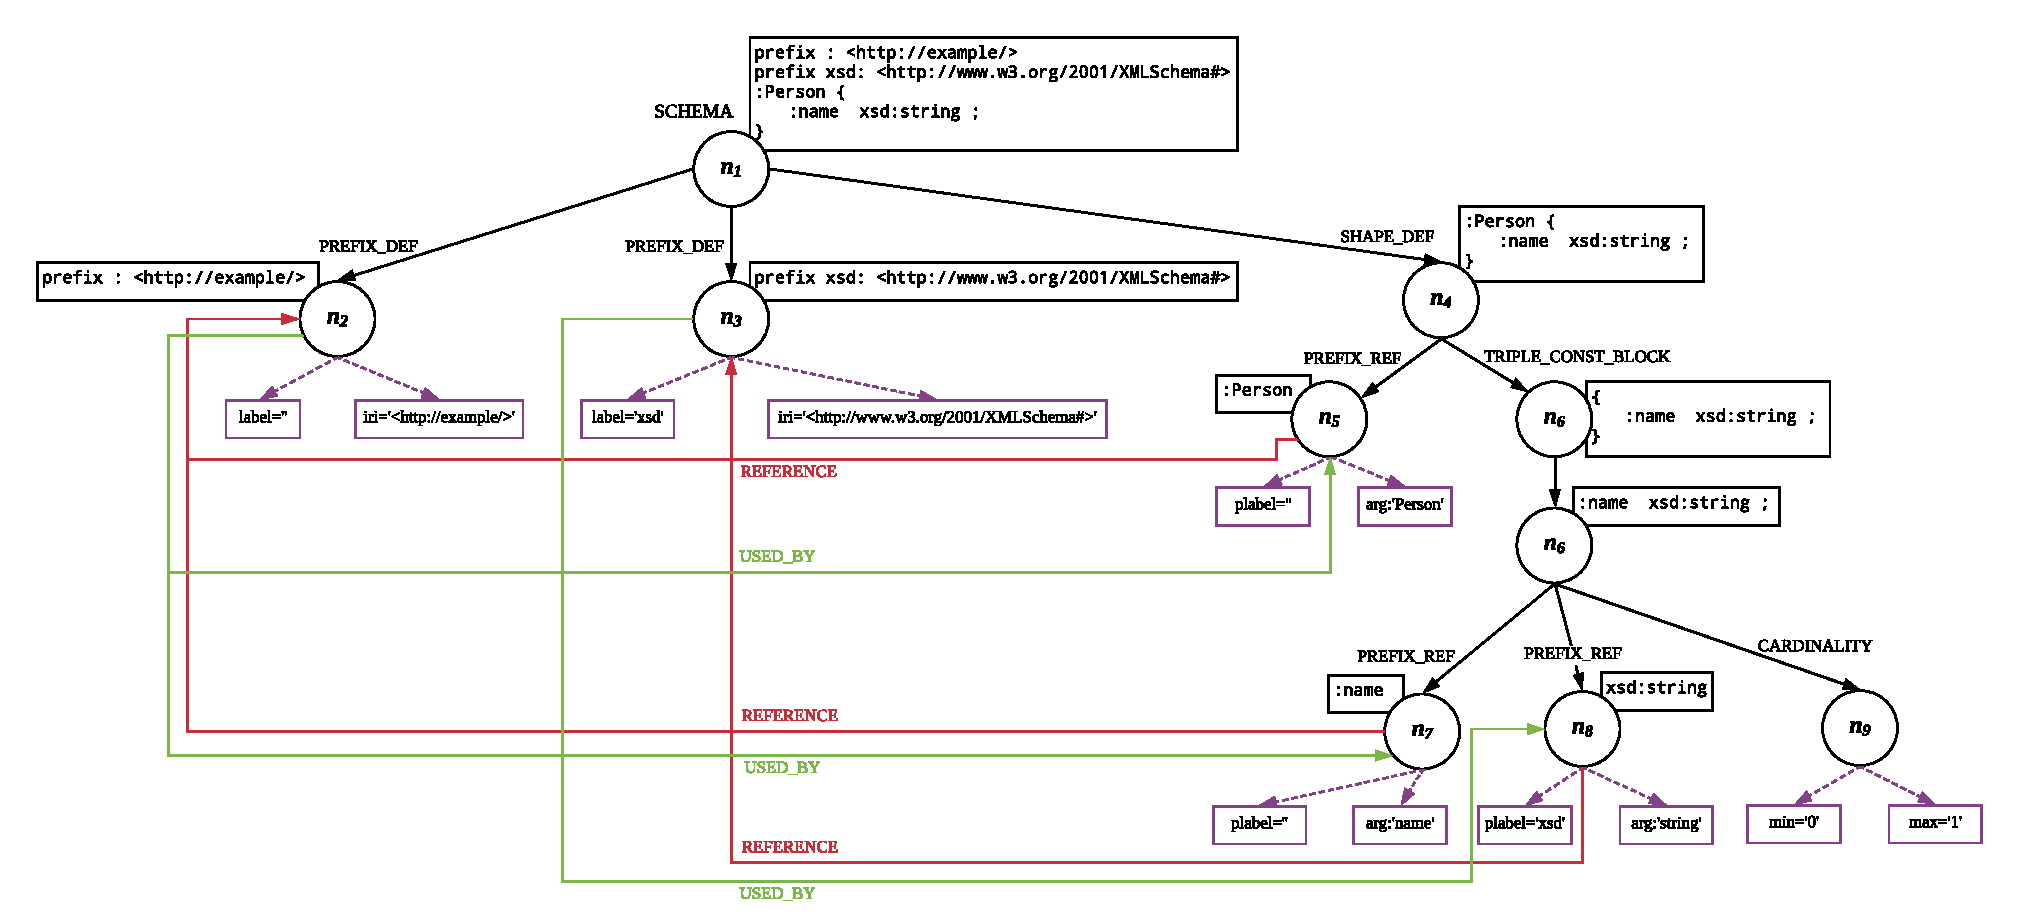
\includegraphics[width=\textwidth]{images/shex-lite-sema-anal.pdf}
    \centering
    \caption[Abstract Syntax Tree produced after validation and transformations]{Abstract Syntax Tree produced after validation and
    transformations.}
    \label{fig:shex-lite-sema-anal}
\end{figure}

Once we have the representation modeled and this representation is capable of expressing all the assumptions of our language,
we can begin to apply validators on our structure. For example if we wanted to find broken references we could go to the nodes
that are a reference to definitions like nodes $n_{\:5,\:7\:and\:8}$ and check that there is indeed a valid reference for each of them.

Furthermore, we can even analyze how many times a definition is used by a reference so that we can launch messages warning the end user
in some cases, such as when a prefix is not used.

\section{Implementation}
As proof of concept of the previous proposal we offer an implementation of the three components, the parser, the sintactic analyzer
and the semantic parser. The implementation is defined in the same way as the structure, in three parts. We will now explore each
of those parts and their responsibilities separately.

\subsection{Parser}
As previously discussed, the function of the parser is to extract a syntactic tree from the diagrams that we can analyze.
For this purpose we decided to use the Antlr tool \cite{parr1995antlr}. This tool is capable of generating sintactic analyzers
from grammars defined in its own syntax. However, this tool is focused on completely processing the syntax tree and producing
only the abstract syntax tree. Therefore we had to use a modification of the original ShEx micro Compact Syntax syntax so that
Antlr would produce a tree with all the syntactic content. This also does offer the flexibility that in the future if we want to
implement any additional syntactic validation we simply have to do it on the tree that the parser generates for
us and not on the Antlr code.

\subsection{Sintactic Analizer}
The sintactic analyzer has the responsibility to validate that the parser produced syntax tree is correct and to build the abstract syntax
tree as well. To do this, it uses the same mechanism. Through the visitor pattern we go through our syntax tree. Each implementation
of this visitor has a purpose, for example an implementation can go through a few specific nodes to validate them syntactically
while another can go through them in order to build the AST. \cref{fig:checker-example} shows an example of how a sintactic check is
implemented.

\begin{figure}
    \begin{lstlisting}[language=Java,numbers=left,basicstyle=\ttfamily\scriptsize]
override def visitConstraint_triple_expr(...) {
  if(/*No trailing semicolon*/)
    //Warn user about this bad practice
}
    \end{lstlisting}
    \caption[Checker implementation for missing semicolons warning generation]{Checker implementation for missing semicolons warning generation.}
    \label{fig:checker-example}
\end{figure}

The AST construction stage is very delicate since for each generated node we have to include as much context information as possible
so that when an error is detected in the tree we can identify not only the cause but also the position, the origin, the rest of the
affected nodes and therefore offer a content-rich error message. Regarding our implementation, for each node we save the following
context information:
\begin{itemize}
    \item \textbf{Source file path.} Represents the path to the source file where the node was generated.
    \item \textbf{Line.} The line in the source file where the node was generated.
    \item \textbf{Column.} The column in the source file where the node was generated.
    \item \textbf{Token interval.} The interval \textit{(start, end position)} of tokens from the source file that generated the node.
    \item \textbf{Content.} The content of the node as plain text. \cref{fig:shex-lite-sema-anal} is very representative of this. 
    \item \textbf{Parent node.} A pointer to the parent node.
    \item \textbf{Children nodes.} A list of pointers to all the children nodes.
\end{itemize}

\cref{fig:shex-lite-node-info} represents this information inside each node. Our default implementation only looks for the
following extra syntactic pattern to the other implementations seen in \cref{ch:current-analyzers-analysis}: shape expressions whose last
triple constraint does not contain the semicolon ending character. In case we find this pattern, we inform the event manager
that a notice has been found that must be passed on to the user, \cref{fig:sin-err-example}.

\begin{figure}
    \begin{lstlisting}[numbers=left,basicstyle=\ttfamily\scriptsize]
warning[W005]: missing semicolon
--> ../../test/assets/input_correct_java_schema_user_car_1.shexl:8:23
    |
8   | :knows      @:User *
    |                      ^ semicolons are not compulsory in the last triple constraint,
                             but its usage its encouraged as otherwise your code wont be
                             following shape expressions specification.
    \end{lstlisting}
    \caption[Sintactic warning produced by the proposed sintactic analyzer]{Sintactic warning produced by the proposed sintactic analyzer.}
    \label{fig:sin-err-example}
\end{figure}

\begin{figure}
    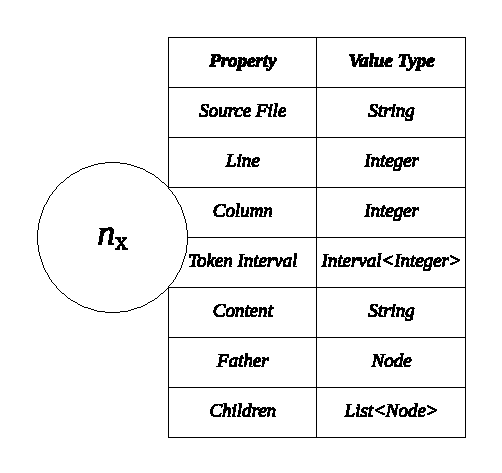
\includegraphics[scale=0.7]{images/shex-lite-node-table.pdf}
    \centering
    \caption[Common information stored at any AST node]{Common information stored at any AST node.}
    \label{fig:shex-lite-node-info}
\end{figure}

\subsection{Semantic Analizer}
Recall that the semantic analyzer takes the generated AST, runs it in search of errors and transforms it in such a way that
it emits a graph that corresponds to the intermediate language. We can separate semantic analysis into two phases, a first
one in which we transform our syntactic tree, adding possible relationships. And a second phase in which we analyze existing
and created relationships.

\subsubsection{Tree transformations}
In the case of our syntax the semantic relations that we find is the linking of a reference to its definition and the opposite
direction to indicate that a definition is being referenced by a node. The transformations are listed bellow:

\begin{itemize}
    \item \textbf{Linking prefix definition with prefix references.} Prefix references occurs when a node describes itself as
    the composition of a prefix and an argument. The idea is that the prefix subtitute the IRI, but must be linked as any
    prefix reference needs to point to an existing definition.
    \item \textbf{Linking base definition with base references.} Some nodes are defined as relative IRIs to the base definition
    and therefore need to be linking to them in order to be able to get that base IRI.
    \item \textbf{Linking shape definition with a shape reference.} Shape definitions can be used at the \texttt{start} definition
    to point the deafult shape or as type constraints in the triple constraints. At any of those points shape references must
    exist within the scope of an schema.
\end{itemize}

\subsubsection{Tree relations analysis}
For this purpose, the semantic analizer defines the visitor pattern on the nodes of the abstract syntax tree so that each of the different
analysis is done with a tree visiting implementation. Some of the 

\section{Sintactic and Semantic Error and Warnings Detected}

\subsection{Not trailing semicolon at last triple constraint}

\subsection{Prefix not defined}

\subsection{Shape not defined}

\subsection{Prefix overriden}

\subsection{Shape overriden}

\subsection{Unused prefix definition}

\subsection{Base set but not used}